\documentclass[journal,12pt,twocolumn]{IEEEtran}
\usepackage{hyperref}
\usepackage{amsmath}
\usepackage{mathtools}
\title{Assignment 4}
\author{JARPULA BHANU PRASAD - AI21BTECH11015}
\date{April 2022}
\newcommand\Mycomb[2][^n]{\prescript{#1\mkern-0.5mu}{}C_{#2}}
\begin{document}
\maketitle
\noindent \Large\underline{Download codes from}:\\
\noindent \large Download python code from - \href{https://github.com/jarpula-Bhanu/Assignment-4/blob/main/codes/probability.py}{Python}\\ Download latex code from - \href{https://github.com/jarpula-Bhanu/Assignment-4/blob/main/Assignment4.tex}{Latex}
\section{\large\underline{Problem-CBSE-9th Q)example 2}}
\large \noindent Q)Two coins are tossed simultaneously 500 times, and we get
\begin{align*}
Two \hspace{2mm} heads : 105 \hspace{2mm} times \\
One \hspace{2mm} head : 275 \hspace{2mm} times \\
No \hspace{2mm} head : 120 \hspace{2mm} times
\end{align*}
Find the probability of occurrence of each of these events.

\section{\large\underline{Solution}}
\noindent Let the random variable $X$ $\in$ \{0,1,2\} denote the number of heads in the coin-tossing experiment.\\ 
Now,
\begin{align}
Pr(X = i) = \frac{n(X = i)}{\sum_{i=0}^2 n(X = i)}
\end{align}
Where $i$ $\in$ \{0,1,2\} and $n(X = i)$ is the frequency of getting $i$ heads.\\
Also,\\ Number of times 2 coins were tossed = 500
\begin{align}
&\implies \sum_{i=0}^2 n(X = i) = 500
\end{align}
Probability of getting zero heads
\begin{align}
Pr(X = 0) = \frac{120}{500} = 0.24
\end{align}
Probability of getting one head
\begin{align}
Pr(X = 1) = \frac{275}{500} = 0.55
\end{align}
Probability of getting two heads
\begin{align}
Pr(X = 2) = \frac{105}{500} = 0.21
\end{align}
\begin{figure}[h] 
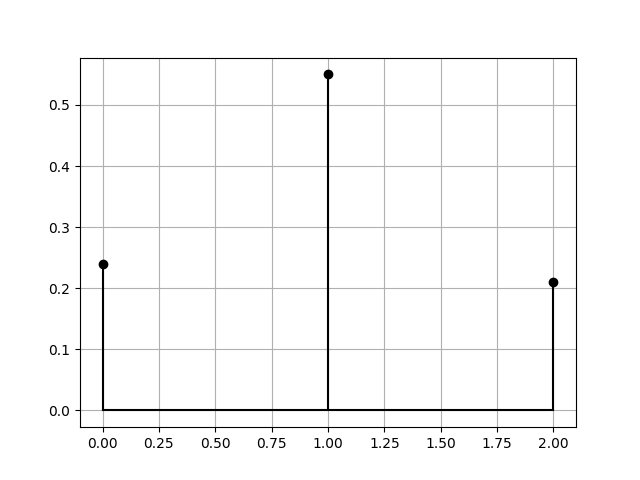
\includegraphics[width=\columnwidth] 
{Figure_1}
\caption{Plot of PMF using above data}
\label{fig:a}
\end{figure}

\noindent \underline{Now considering fair coins:} Let probability of getting a head be a success and equal to $p$ and probability of getting a tail be a failure and equal to $q$ where $p+q$ = 1. We can express this as a binomial distribution
\begin{align}
\sum_{i=0}^n Pr(X=i) = \sum_{i=0}^n \Mycomb[n]{i} (p)^{i} (1-p)^{n-i}
\end{align}
Where $n$ = 2 for 2 coins. Therefore,
\begin{align}
Pr(X = i) = \Mycomb[2]{i} (p)^{i} (q)^{2-i}
\end{align}
For fair coins,
\begin{align}
p = \frac{1}{2} \hspace{5mm} and \hspace{5mm} q = \frac{1}{2}
\end{align}
Therefore,
\begin{align}
Pr(X=0) = \Mycomb[2]{0} \Big(\frac{1}{2}\Big)^{0} \Big(\frac{1}{2}\Big)^{2} = \frac{1}{4} \\
Pr(X=1) = \Mycomb[2]{1} \Big(\frac{1}{2}\Big)^{1} \Big(\frac{1}{2}\Big)^{1} = \frac{1}{2} \\
Pr(X=2) = \Mycomb[2]{2} \Big(\frac{1}{2}\Big)^{2} \Big(\frac{1}{2}\Big)^{0} = \frac{1}{4} 
\end{align}
\begin{figure}[h] 
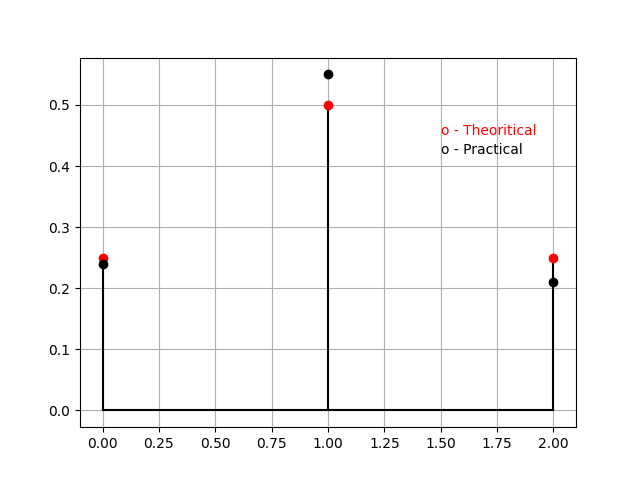
\includegraphics[width=\columnwidth] 
{Figure_2}
\caption{Comparison of theoretical and practical PMF plots }
\label{fig:b}
\end{figure}
\end{document}